%&pdflatex
\section{Scrittura su CD/DVD}
Per scrivere un file immagine ISO su un CD o un DVD (un CD è sufficiente per la netinst di Debian) da Microsoft Windows, si può usare un tool come \texttt{ImgBurn}:

\begin{graybox}
	http://www.imgburn.com/index.php?act=download
\end{graybox}

Inseriamo un CD/DVD vuoto. All'apertura ImgBurn si presenterà come in Figura \vref{fig:imgburn}.

\begin{figure}[ht]
	\centering
	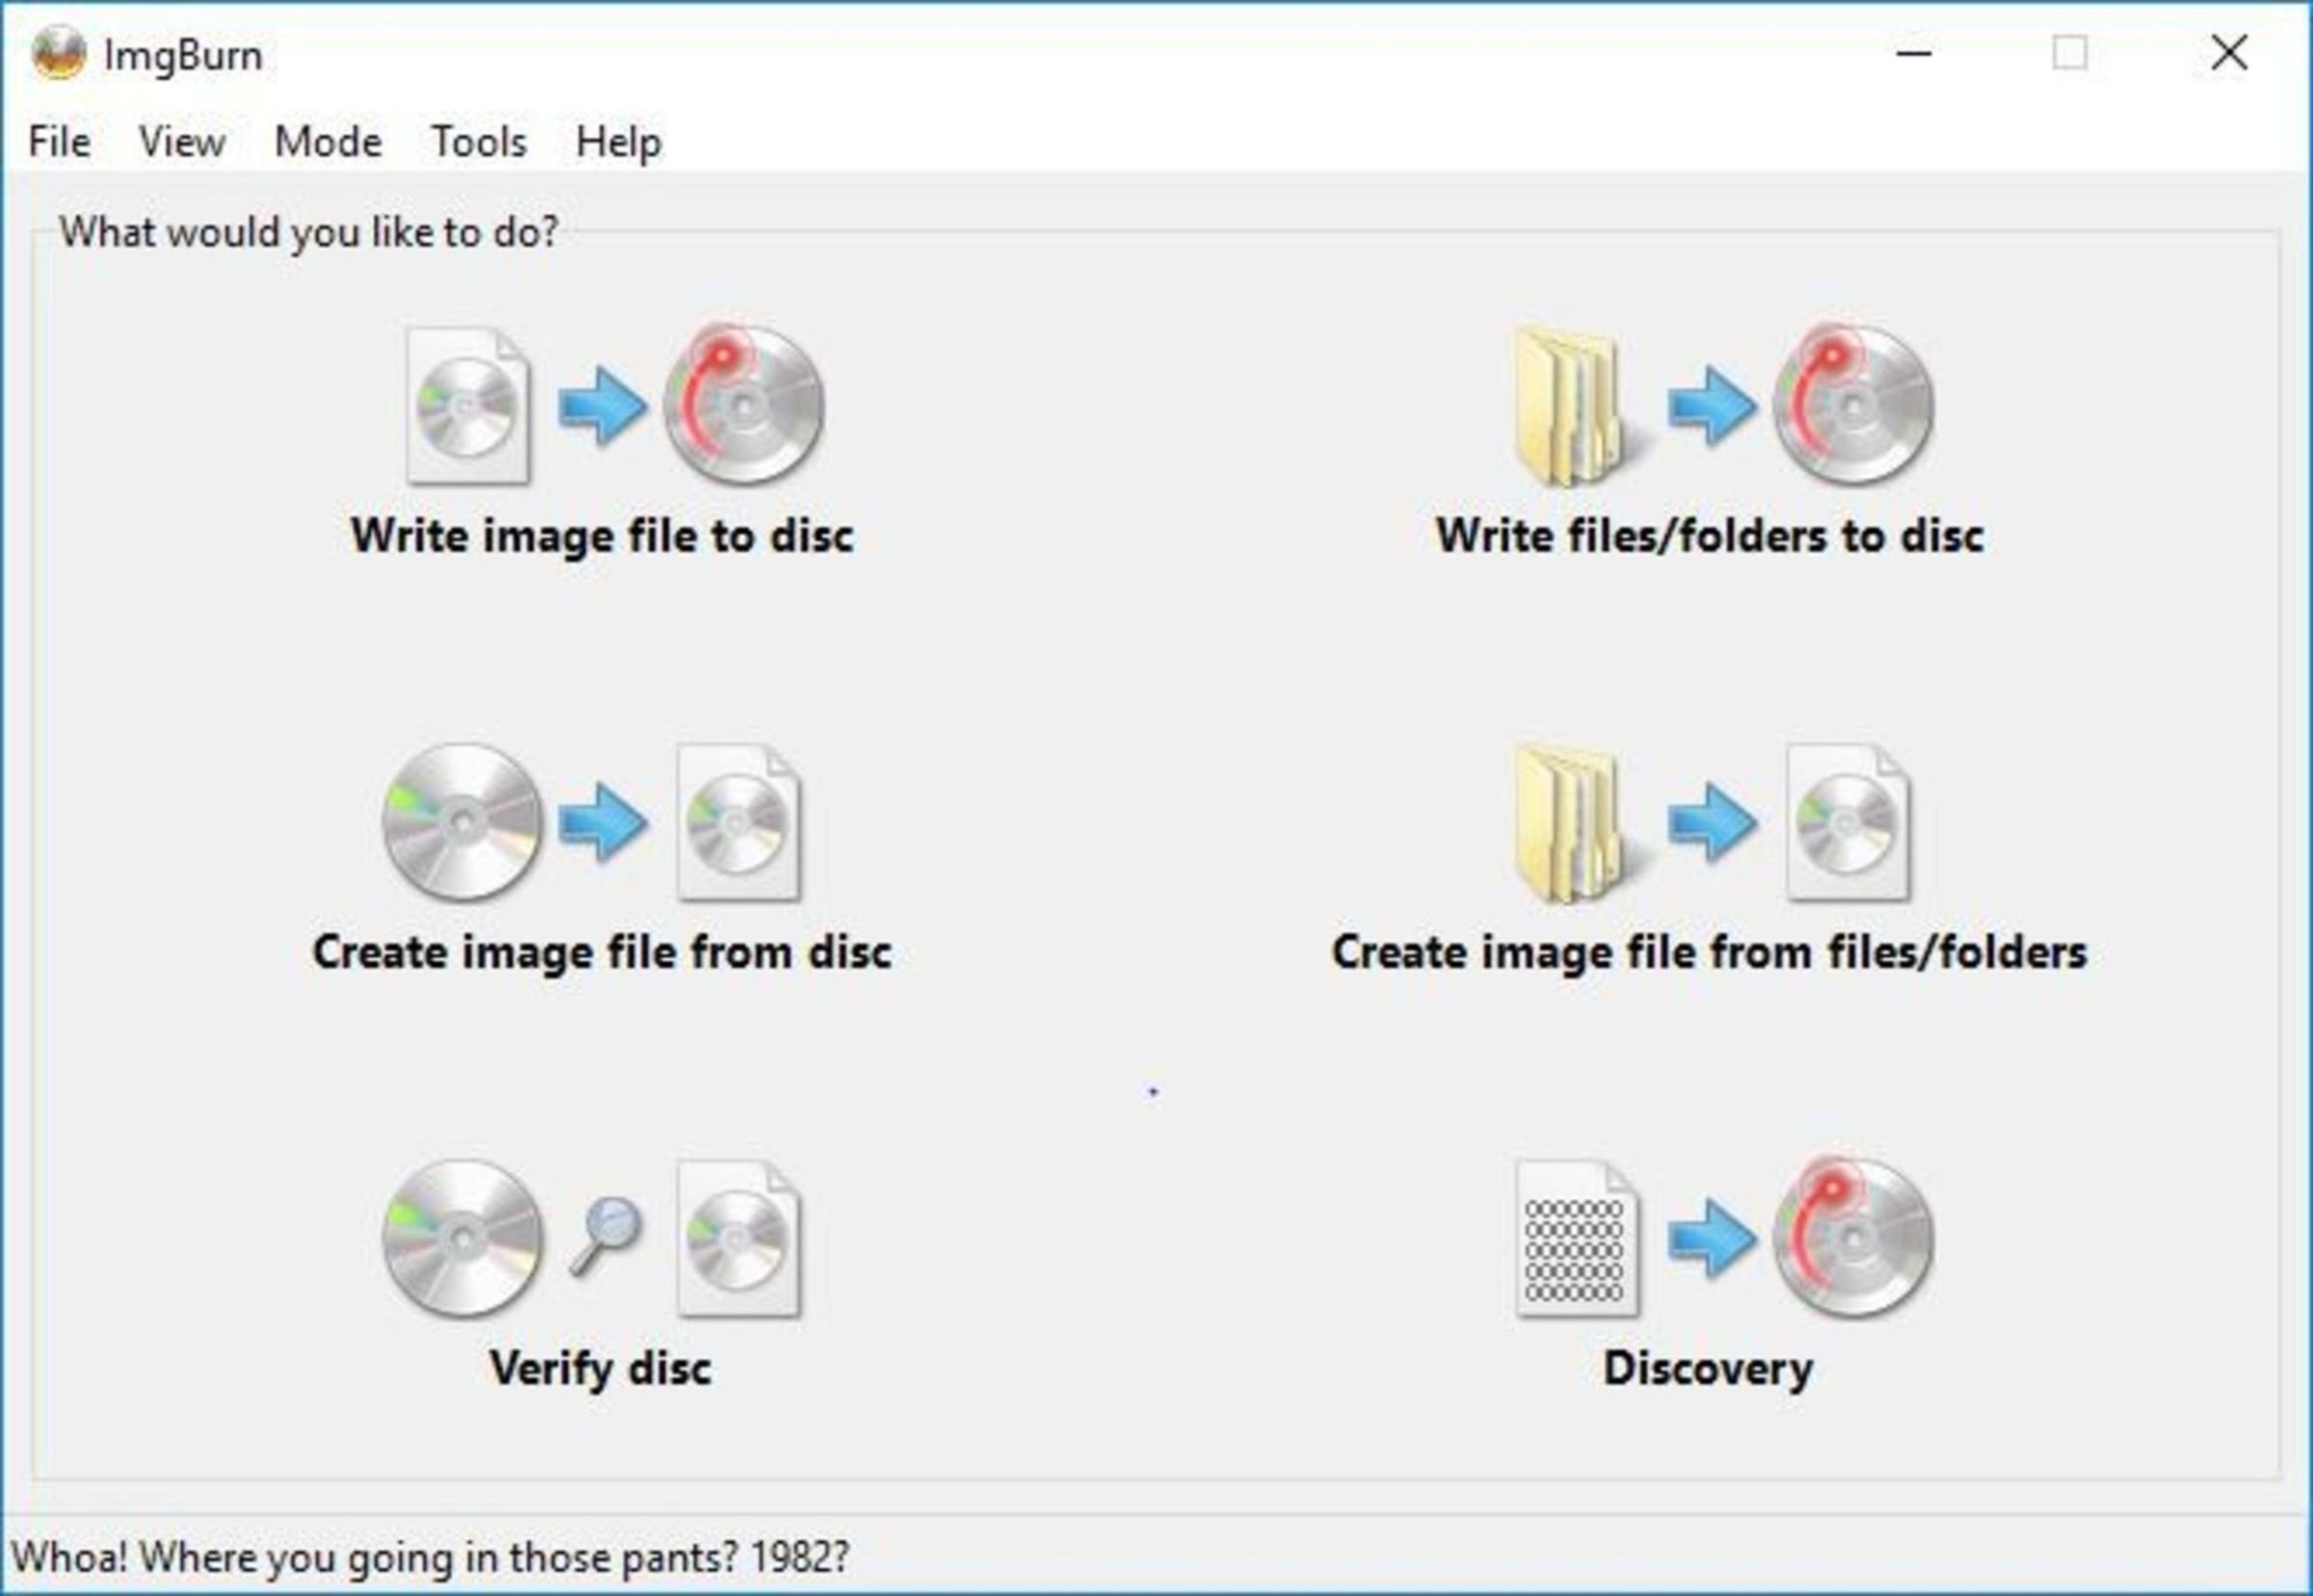
\includegraphics[resolution=600]{imgburn}
	\caption{Prima schermata di ImgBurn}
	\label{fig:imgburn}
\end{figure}

Scegliamo \texttt{Write image file to disc} (\texttt{Scrivi un file imma\-gine su disco}) e comparirà la schemata mostrata in Figura \vref{fig:burning}.

\begin{figure}[ht]
	\centering
	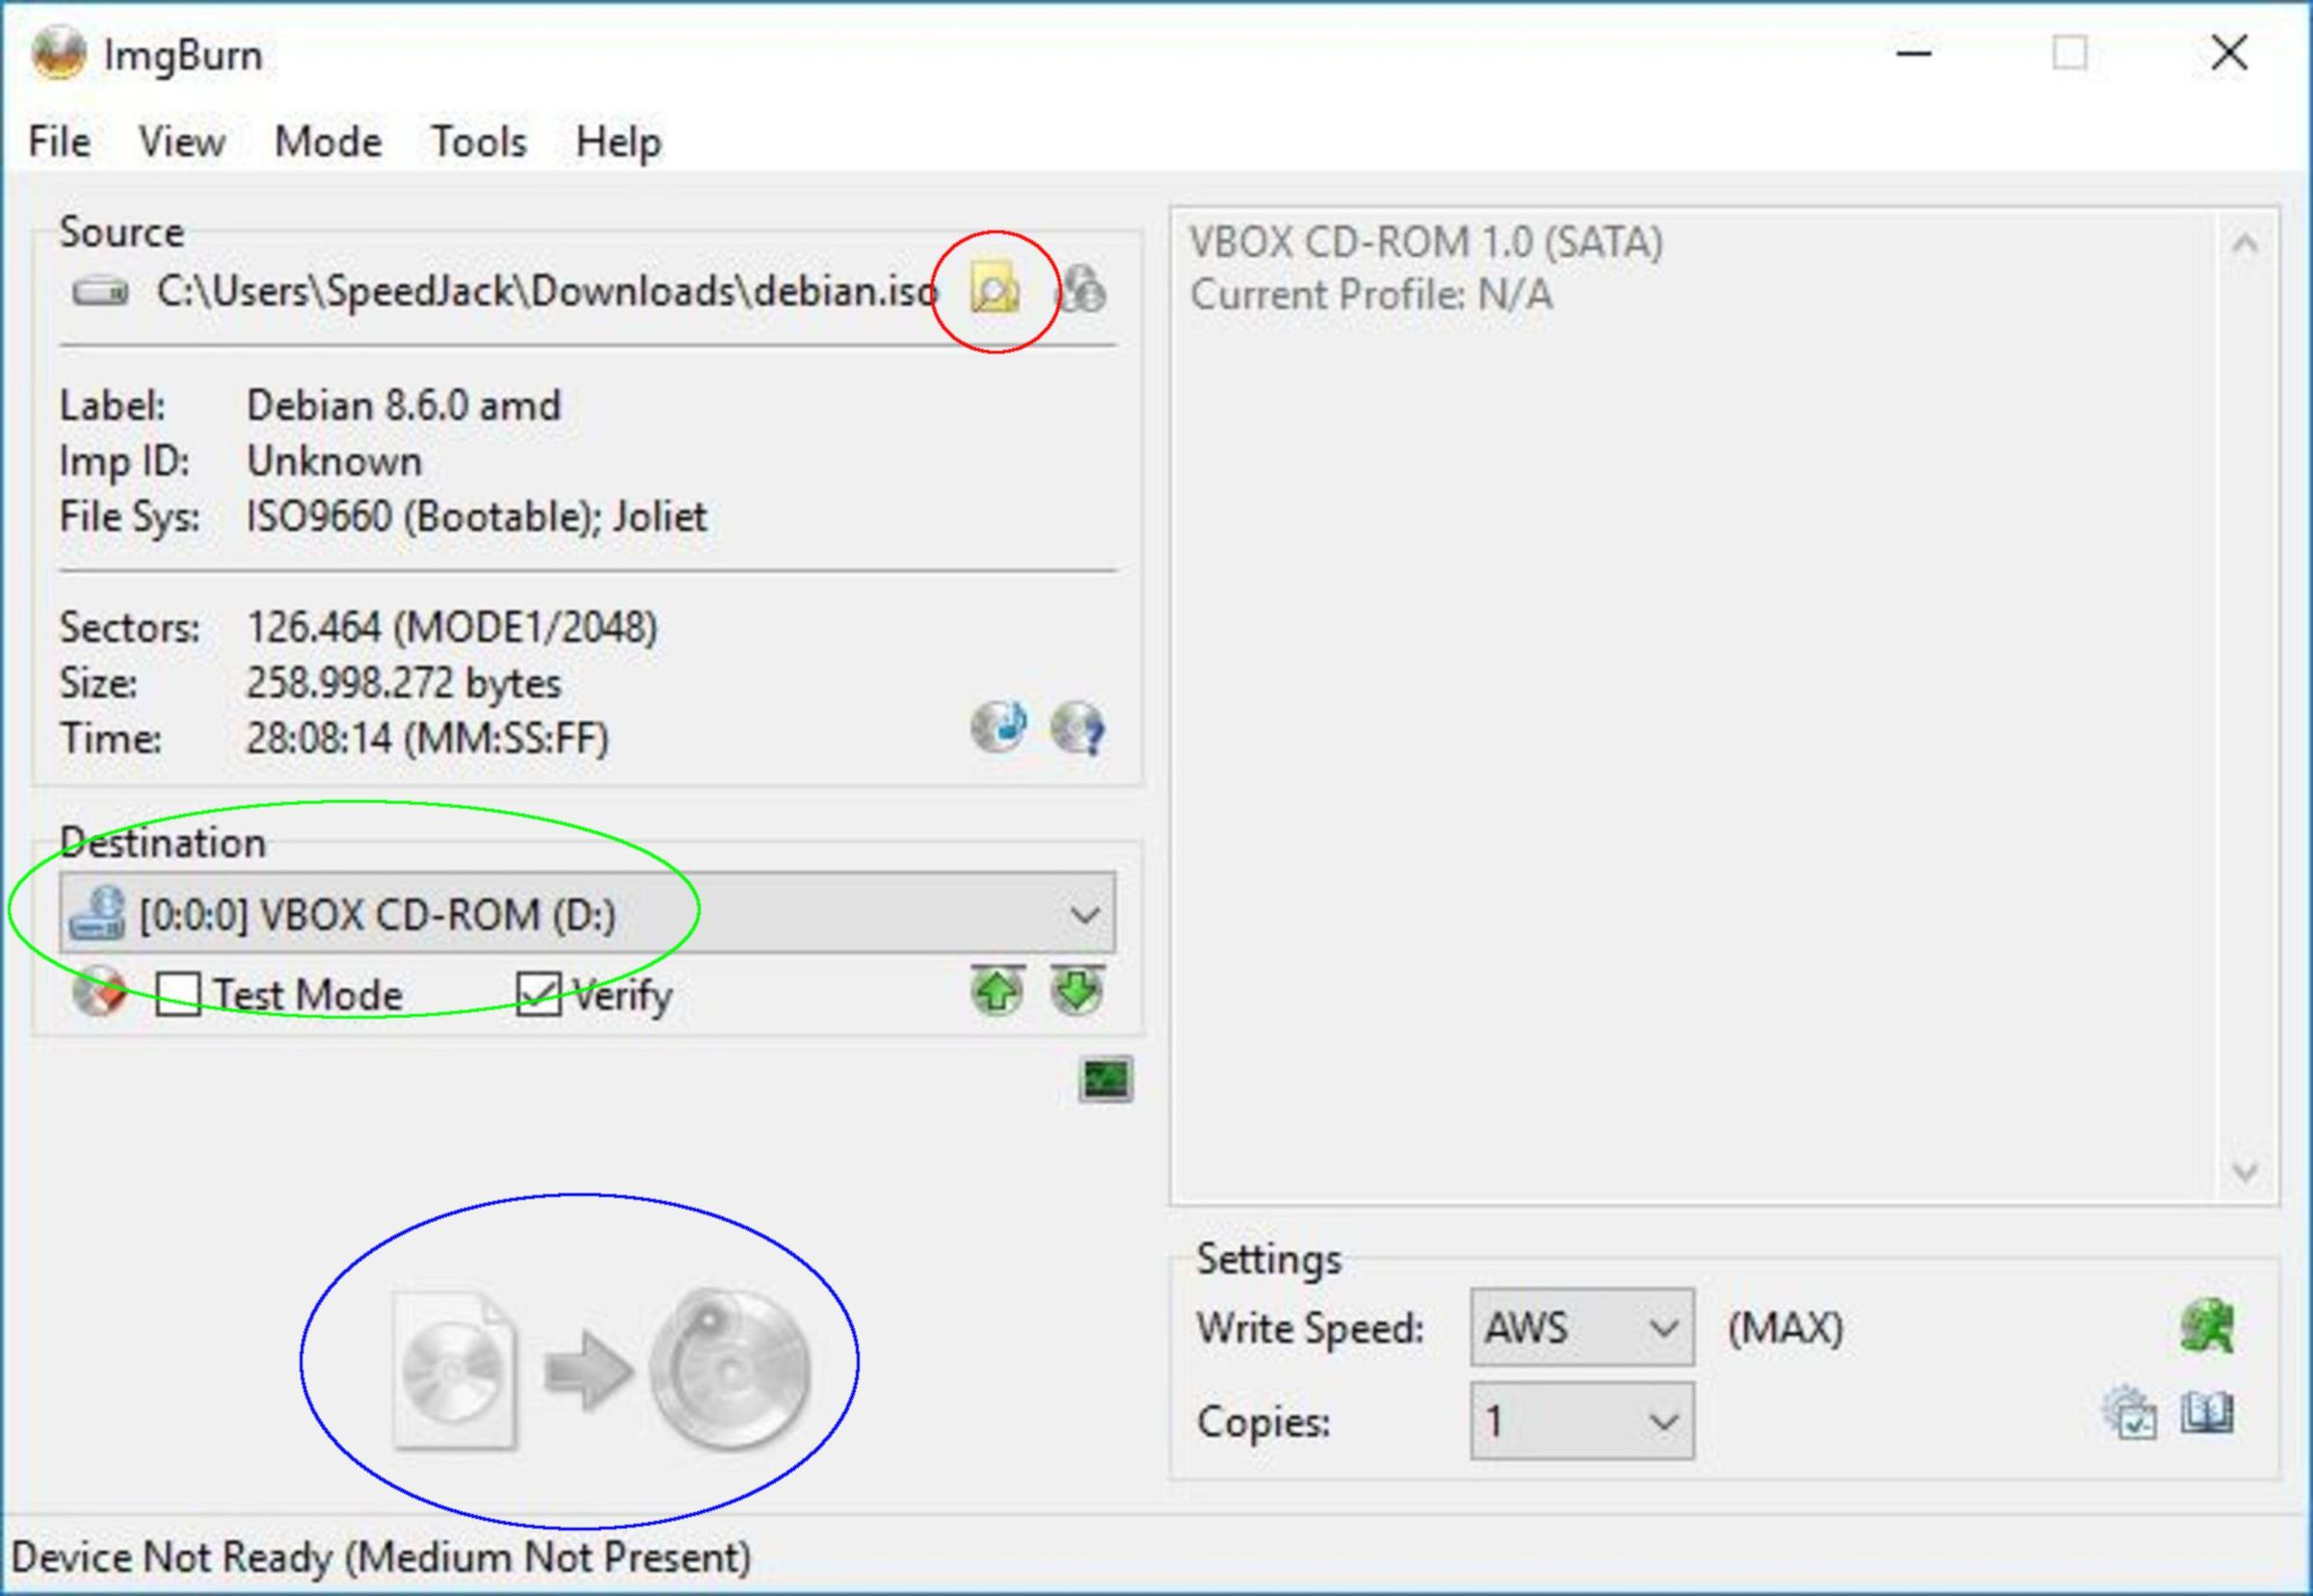
\includegraphics[resolution=600]{burning}
	\caption{Scrittura di un'immagine su disco con ImgBurn}
	\label{fig:burning}
\end{figure}

In alto, cliccando sul piccolo simbolo cerchiato in rosso, selezioniamo il file immagine ISO di Debian. In basso, assicuriamoci che il campo cerchiato in verde sia corretto (deve indicare il CD/DVD vuoto che abbia appena inserito). Infine, clicchiamo sul grosso tasto in basso (cerchiato in blu).

A questo punto ImgBurn inizierà la scrittura. Una volta terminata la scrittura è possibile procedere con il paragrafo \vref{sec:bios-uefi}.
